%=========================================================================
% (c) Michal Bidlo, Bohuslav Křena, 2008

\chapter{Úvod}
Úvod tejto bakalarskej prace bude popisany az nakoniec \footnote{Viz Zasady pisania odbornych prac}.

\begin{itemize}
\item prerekvizita je dadydadydaaa
\item cluster je toto
\item a~este tam mame nieco ine
\end{itemize}

\subparagraph{aa1}
aaa1
\subparagraph{aa2}
aaa2

TOto je \textbf{Tucny text} uprostred  normalneho textu.

Toto je \emph{Emph text} uprostred normalneho textu.

\chapter{Testovanie softvéru}
V~nasledujúcej kapitole sú stručne zhrnuté teoretické vedomosti o~testovaní softvéru.
Kapitola \ref{sekcia:typy_testovania} popisuje, prečo je testovanie softéru dôležité a~aké rôzne typy
testovania softvéru sa dnes používajú.
V~kapitole \ref{sekcia:testovanie_v_praxi} si popíšeme, ako sa automaticky testuje softvér vo firme Acision a~aké nástroje táto firma využíva.
Nakoniec kapitola \ref{sekcia:planovac} popisuje plánovač testov, ktorý firma Acision každodenne používa 
pri testovaní rôznych typov softvéru, ktorý firma vyvíja. 
Cieľom tejto bakalárskej práce je úprava tohto plánovača tak, aby podporoval distribúciu testov na viaceré systémy,
a~tým urýchlil čas potrebný na otestovanie softvéru danou sadou testov. 

\section{Typy testovania softvéru} \label{sekcia:typy_testovania}
Testovanie softvéru je v~dnešnej dobe jedným z~kľúčových faktorov v~IT sfére.
Podľa štandardu IEEE 1059 \cite{Ieee} je testovanie proces analýzy softvéru a~detekovanie rozdielností medzi 
existujúcimi a~požadovanými podmienkami a~vyhodnocovaní vlastností testovaného softvéru.
Viaceré zdroje avšak pojem testovania softvéru definujú inak.
Dokument \cite{Swebok} definuje pojem testovania softvéru ako {\it dynamickú} verifikáciu správania programu voči {\it očakávanému} správaniu programu na {\it konečnej} vzorke
testov, vhodne {\it zvolenej} zo zvyčajne nekonečného množstva možných prípadov použitia.
Pressman v~dokumente \cite{Pressman} prehlásil, že testovanie softvéru je kritickým prvkom zabezpečenia kvality softvéru, ktorý má jedinú primárnu úlohu, a~to násť v~ňom chyby.  

Existujú rôzne spôsoby delenia testovania softvéru. Jedno z~hlavných delení je delenie podľa spôsobu testovania.
Toto rozdelenie vychádza z~toho, či je potrebné k~prevedeniu testu daný softvér spustiť, alebo nie.
\subsection*{Statické testovanie}
Statické testovanie je testovanie, ktoré nevyžaduje beh softvéru. Statická analýza sa snaží odhaliť niektoré
programátorské chyby ako napríklad syntaktické chyby, neicializované premenné, nesprávna práca s~pamäťou, delenie nulou, opakované zavretie súboru a~ďalšie. 
Medzi statické testovanie patrí napríklad revízia kódu alebo použitie niektorého nástroja pre statické testovanie, napríklad syntaktický analyzátor, sémantický
analyzátor, analyzátor závislostí, atď. Statické testovanie môže byť manuálne alebo automatické. Tento typ testovania je možný v~ľubovolnej fáze vývoja softvéru.
\subsection*{Dynamické testovanie}
Dynamické testovanie vyžaduje beh testovaného softvéru. Dynamické testovanie môže produkovať výsledky, ktoré nie sú so statickou analýzou možné, alebo 
by boli použitím statického testovania časovo náročné. Tento typ testovania vyžaduje spustiteľnú verziu vyvýjaného softvéru.
\\
\\
Medzi ďalšie delenie patrí delenie testovania podľa spôsobu vykonávania testov:
\subsection*{Manuálne testovanie}
Pri manuálnom testovaní vykonáva test používateľ priamou interakciou s~testovaným produktom. 
Tento typ testovania sa používa,pokiaľ test potrebuje ľudské ohodnotenie alebo úsudok.

\subsection*{Automatické testovanie}
Automatické testovanie je prevádzané strojom.
Tento typ testovania sa zavádza väčšinou do rozsiahlych projektov.
Využíva sa pri opakovanom spúsťaní veľkého množstva testov, alebo testov s~veľkými množstvami dát.
Pri automatickom testovaní sa využíva nejaký automatizovaný nástroj, pričom môže ísť o~nástroje 
pre vykonávanie testov, alebo o~nástroje pre správu testov.
\\
\\
Trocha odlišne sa pristupuje k~deleniu testov na základe toho, aké znalosti máme o~testovanom produkte.
Môže ísť o:
\subsection*{Testovanie pomocou bielej skrinky}
Tento typ testovania vyžaduje prístup k~zdrojovému kódu softvéru. Na základe znalosti zdrojového kódu sa potom vytvárajú testy.
Testovanie pomocou bielej skrinky však nemusí odhaliť neimplementované časti systému, alebo chýbajúce požiadavky.
\subsection*{Testovanie pomocou čiernej skrinky} \label{sekcia:cierna_skrinka}
Táto metóda nevyžaduje znalosť zdrojového kódu testovaného softvéru počas vytvárania testov.
Pri návrhu testov sa používa externý pohľad na testovaný softvér. 
Produkt berieme ako čiernu skrinku, do ktorej sa nevieme pozrieť.
O~tejto čiernej skrinke vieme len to, ako sa chová navonok a~ako vyzerá.
Pri tomto type testovania sa zameriavame na vstupy a~výstupy programu bez znalosti toho, ako je naimplementovaný.
\subsection*{Testovanie pomocou sivej skrinky}
Testovanie pomocou sivej skrinky je forma testovania niekde medzi bielou a~čiernou skrinkou. 
Využívajú sa v~nej limitované vedomosti o~implementácií testovaného softvéru.
Nemáme napríklad k~dispozícií celý zdrojový kód, ale iba dizajn softvéru alebo databázu.
\\
\\
Testovanie softvéru môže byť zvyčajne vykonávané na rôznych úrovniach 
procesu vývoja alebo údržby softvéru. Cieľ testu môže byť rôzny: od jedného
modulu, cez skupinu modulov, alebo celého systému.
Toto delenie je na základe úrovní testovania softvéru a~vyzerá nasledovne:
\subsection*{Unit testy}
Tieto testy verifikujú funkcionalitu softvéru v~častiach, ktoré sú testovateľné oddelene.
Unit testy sú definované presnejšie v~štandarde IEEE1008-87 \cite{Ieee_unit}.
\subsection*{Integračné testovanie}
Integračné testovanie je proces, v~ktorom sa verifikuje interakcia medzi viacerými softvérovými komponentami.
\subsection*{Systémové testovanie}
Systémové testovanie sa zaoberá správaním celého systému. Počas systémového testovania sa aplikácia testuje ako celok,
a~preto je toto testovanie vhodné pre neskoršie fázy vývoja.
\subsection*{Akceptačné testovanie}
Testuje správanie systému voči požiadavkám zákazníka. Akceptačné testy overujú to, ako je daný softvér 
schopný byť nasadený do ostrej prevádzky, a~typicky sú súčasťou prevzatia softvéru zákazníkom.

Testovanie môže byť cieľené na verifikovanie rôznych vlastností softvéru. Na základe toho, na akú časť systému je 
testovanie zamerané, môžeme testovanie rozdeliť na:
\subsection*{Inštalačné testovanie}
Toto testovanie overuje, či je vytvorený softvér možné nainštalovať
na cieľové prostredie. Na tento typ testovania sa môžeme pozrieť ako na 
systémové testovanie ovplyvnené viacerými faktormi, ako napríklad hardwarové požiadavky
alebo požiadavky na operačný systém. 
\subsection*{Testovanie výkonu}
Tento typ testovanie je špeciálne zameraný na to, že softvér spĺňa stanovené požiadavky 
na výkon, ako napríklad doba odozvy alebo počet vykonaných operácií za čas. 
\subsection*{Regresné testovanie} \label{sekcia:regresne_testovanie}
Podľa štandardu IEEE610.12 \cite{Ieee_glossary} je regresné testovanie \quotedblbase Selektívne pretestovávanie 
systému alebo komponenty na verifikáciu, že zmeny nespôsobili nechcené efekty a~že systém alebo
komponenta stále spĺňa špefikované požiadavky.\textquotedblleft
Myšlienkou tohoto testovania je overiť to, že nové zmeny do funkcionality systému nezaniesli do systému nové typy chýb.
Bežným spôsobom tohoto testovania je periodické spúšťanie testov vytvorených v~minulosti a~kontrolovanie, či sa zmenilo správanie
systému, a~či sa chyby opravené v~minulosti znovu neprejavili.
\subsection*{Testovanie použiteľnosti}
Testovanie použitelnosti overuje, aké zložité je pre koncového používateľa pracovať s~daným softvérom.
Toto testovanie overuje taktiež prácu s~dokumentáciou, alebo napríklad schopnosť zotavenia sa z~chyby. 

Uvedené delenia testovania a~ich typy patria medzi najzákladnejšie. 
Existuje ešte niekoľko spôsobov delenia testovania softvéru, ktoré v~tejto kapitole nie sú popísané.

\section{Testovanie softvéru v~praxi} \label{sekcia:testovanie_v_praxi}
V~nasledujúcej kapitole si popíšeme, ako môže byť riešené testovanie komerčného softwaru v~praxi.
Firma Acision\footnote{http://www.acision.com/}, pre ktorú je táto bakalárska práca vytváraná, vyvíja niekoľko komerčných produktov
v~sfére messagingu. Pri produktoch je kladený veľký dôraz práve na testovanie.
Jedným z~najväčších produktov, ktorý firma vyvíja je produkt {\it Message Controller}
\footnote{http://www.acision.com/services/messaging-infrastructure/message-controller} (ďalej len MCO).
Táto bakalárska práca je zameraná pre potreby tohoto produktu a~jeho derivátov.
MCO je komerčný systém, ktorý je na trhu dostupný už niekoľko rokov, a~preto sú hodnoty uvedené v~tejto 
bakalárskej práci z~oddelenia maintenance, ktoré je zodpovedné za údržbu systému a~opravovania chýb v~ňom vyskytnutých.
Jednotlivé produkty sú každodenne testované regresnou sadou testov, ktorá v~prípade MCO pozostáva z~asi 1500 testov.

Údržba produktu MCO funguje formou kontinuálnej integrácie\footnote{angl. Continuous integration}.
Kontinuálna integrácia je vývoj softwaru, kedy členovia týmu spájanú ich prácu častejšie.
Obvykle každý člen tímu integruje svoju prácu aspoň raz denne, čo vedie k~niekoľkým integráciám za deň.
Každá integrácia je verifikovaná automatickým buildom a~testami, aby sa detekovali chyby čo najskôr \cite{Continuous_integration}.

V~praxi to zjednodušene prebieha tak, že je vývojárovi pridelený tzv. ticket, ktorý slúži na popis
nájdenej chyby v~systéme. Pomocou verzovacieho systému si vezme aktuálnu verziu zdrojových súborov a~začne nájdenú chybu opravovať.
Po tom, čo vývojár chybu opraví, zmeny do zdrojového kódu mu skontroluje iný vývojár.
Ak so zmenami do zdrojového kódu bude súhlasiť, uložia tieto zmeny do verzovacieho systému.
Týmto spôsobom sa zaisťuje kontinuálna integrácia na strane vývojárov.

Paralelne s~týmto vývojom beží na jednom servery program, ktorý monitoruje zmeny vo verzovacom systéme.
Ak sa nájde nejaká zmena v~zdrojových kódoch, spustí sa automatický preklad a~zdrojové kódy spolu s~dokumentáciou
sa nanovo skompilujú. Vytvorí sa spustiteľná verzia nového systému. Ak sa preklad zdrojových kódov nepodarí, vývojár, ktorý 
danú chybu spôsobil, je na stav upozornený a~môže sa čo najrýchlejšie pustiť do opravy spôsobenej chyby kompilácie.

Z~pohľadu testera je situácia podobná. Testerovi je taktiež pridelený ticket, pomocou verzovacieho systému si zoberie aktuálnu verziu
všetkých testov a~začne pracovať na novom teste, ktorý overí, že vývojár opravil chybu popísanú v~tickete správne.
Ihneď po dokončení testu zaraďuje tento test pomocou verzovacieho systému do aktuálneho repozitára a~vyžiada si
kontrolu napísaného testu. Tester väčšinou pristupuje k~testovanému produktu metódou čiernej skrinky (viď kapitola \ref{sekcia:cierna_skrinka}).

Raz denne (typicky v~noci) sa potom vezme najnovšia spustiteľná verzia systému, a~na tomto systéme sa pustí aktuálna verzia
všetkých dostupných testov. Pomocou regresného testovania (viď kapitola \ref{sekcia:regresne_testovanie}) sa potom overí, či sa zmenou zdrojového kódu nezaniesli do systému nové
chyby. Všetky testy sú plne automatizované a~dynamicky overujú, že testovaný systém splňuje všetky požiadavky.

Týmito postupmi je zaistená kontinuálna integrácia. Implementácií kontinuálnej integrácie 
sa venuje napríklad dokument \cite{Continuous_integration_implementation}. 
Postupnou iteráciou týchto procesov sa dosahuje výsledná kvalita systému. Vačšina testov pristupuje k~testovanému
systému metódou čiernej skrinky, takže tester nepotrebuje znalosť zdrojového kódu, a~môže tak vytvárať testy
ešte pred dokončením samotnej implementácie systému. 

Pre potreby tohto testovania vznikol nástroj, ktorý je schopný zostaviť plán všetkých testov, a~tieto testy postupne vykonať.
Výhodou tohoto nástroja je hlavne to, že je schopný jednoducho zaradiť novovytvorené testy do regresnej sady, ktorá
testuje systém množinou všetkých testov. Postupným pridávaním testov do tejto regresnej sady sa však zvýšil čas potrebný pre otestovanie celého systému.
Regresné testovanie sa časom stalo veľmi časovo náročné, nakoľko čas na otestovanie celého systému sa vyšplhal až 15 hodín a~stále narastal.
Vznikol problém, že počas noci sa nestihol otestovať celý systém a~na začiatku pracovnej doby sa ešte muselo čakať na výsledky regresného testovania.
Pre riešenie tohto problému vznikol nápad vytvorenia rozšíreného plánovača testov, ktorý by bol schopný spúštať testy na viacerých testovacích systémoch.
V~praxi to znamená, že množina všetkých regresných testov sa rozdelí na niekoľko podmnožín, kde každá podmnožina testov sa spustí na samostatnom
testovacom stroji. Týmto spôsobom sme schopní skrátiť čas potrebný pre otestovanie celého systému bez toho, aby sme museli niektoré testy z~regresnej sady 
úplne vypustiť. 

\section{Princíp použitého plánovača testov} \label{sekcia:planovac}
Pre popis rozšírenia plánovača testov si najprv musíme vysvetliť princíp, akým daný plánovač testov funguje.
Pre vysvetlenie tohto princípu si však najprv zavedieme niektoré kľúčové pojmy.
\begin{itemize}
\item \textbf{cluster -} je test, ktorý verifikuje funkčnosť nejakej časti systému. Každý cluster je pomenovaný pomocou prefixu {\it cl\_}. 
\item \textbf{prerekvizita -} je test, ktorý nastavuje nejakú vlastnosť systému na požadovanú hodnotu, prípadne zapína časť systému. 
Každá prerekvizita má svoju vlastnú odrekvizitu a~je pomenovaná pomocou prefixu {\it p\_}.
\item \textbf{odrekvizita -} je test, ktorý vracia zmeny systému spôsobené jej vlastnou prerekvizitou. Každá odrekvizita je pomenovaná
pomocou prefixu {\it u\_}. 
\item \textbf{test -} je cluster, prerekvizita alebo odrekvizita.
\end{itemize}

Plánovač testov je napísaný v~skriptovacom jazyku TCL\footnote{https://www.tcl.tk/}. 
Je špeciálne navrhnutý pre potreby testovania softwaru, ktorý je vysoko konfigurovateľný. 
Využíva oddelenie časti kódu pre samotný test, a~pre konfiguračné zmeny. 
Idea plánovača je taká, že každý test sa rozdelí na prerekvizitu (prípadne viac prerekvizít) a~cluster. Cluster obsahuje zdrojový kód, ktorý verifikuje, že daná
časť systému funguje podľa špecifikácie. Prerekvizita obsahuje zdrojový kód, ktorý mení chovanie systému pre potreby verifikovania funkcionality systému.
Zmena chovania systému môže byť prevádzaná napr. príkazovou riadkou, zmenou konfiguračného súboru a~pod.
Tento princíp usporiadava všetky testy do štruktúry, ktorá je znázornená na obrázku \ref{figure:ukazka_planu}.
\begin{figure}[h]
	\begin{center}
    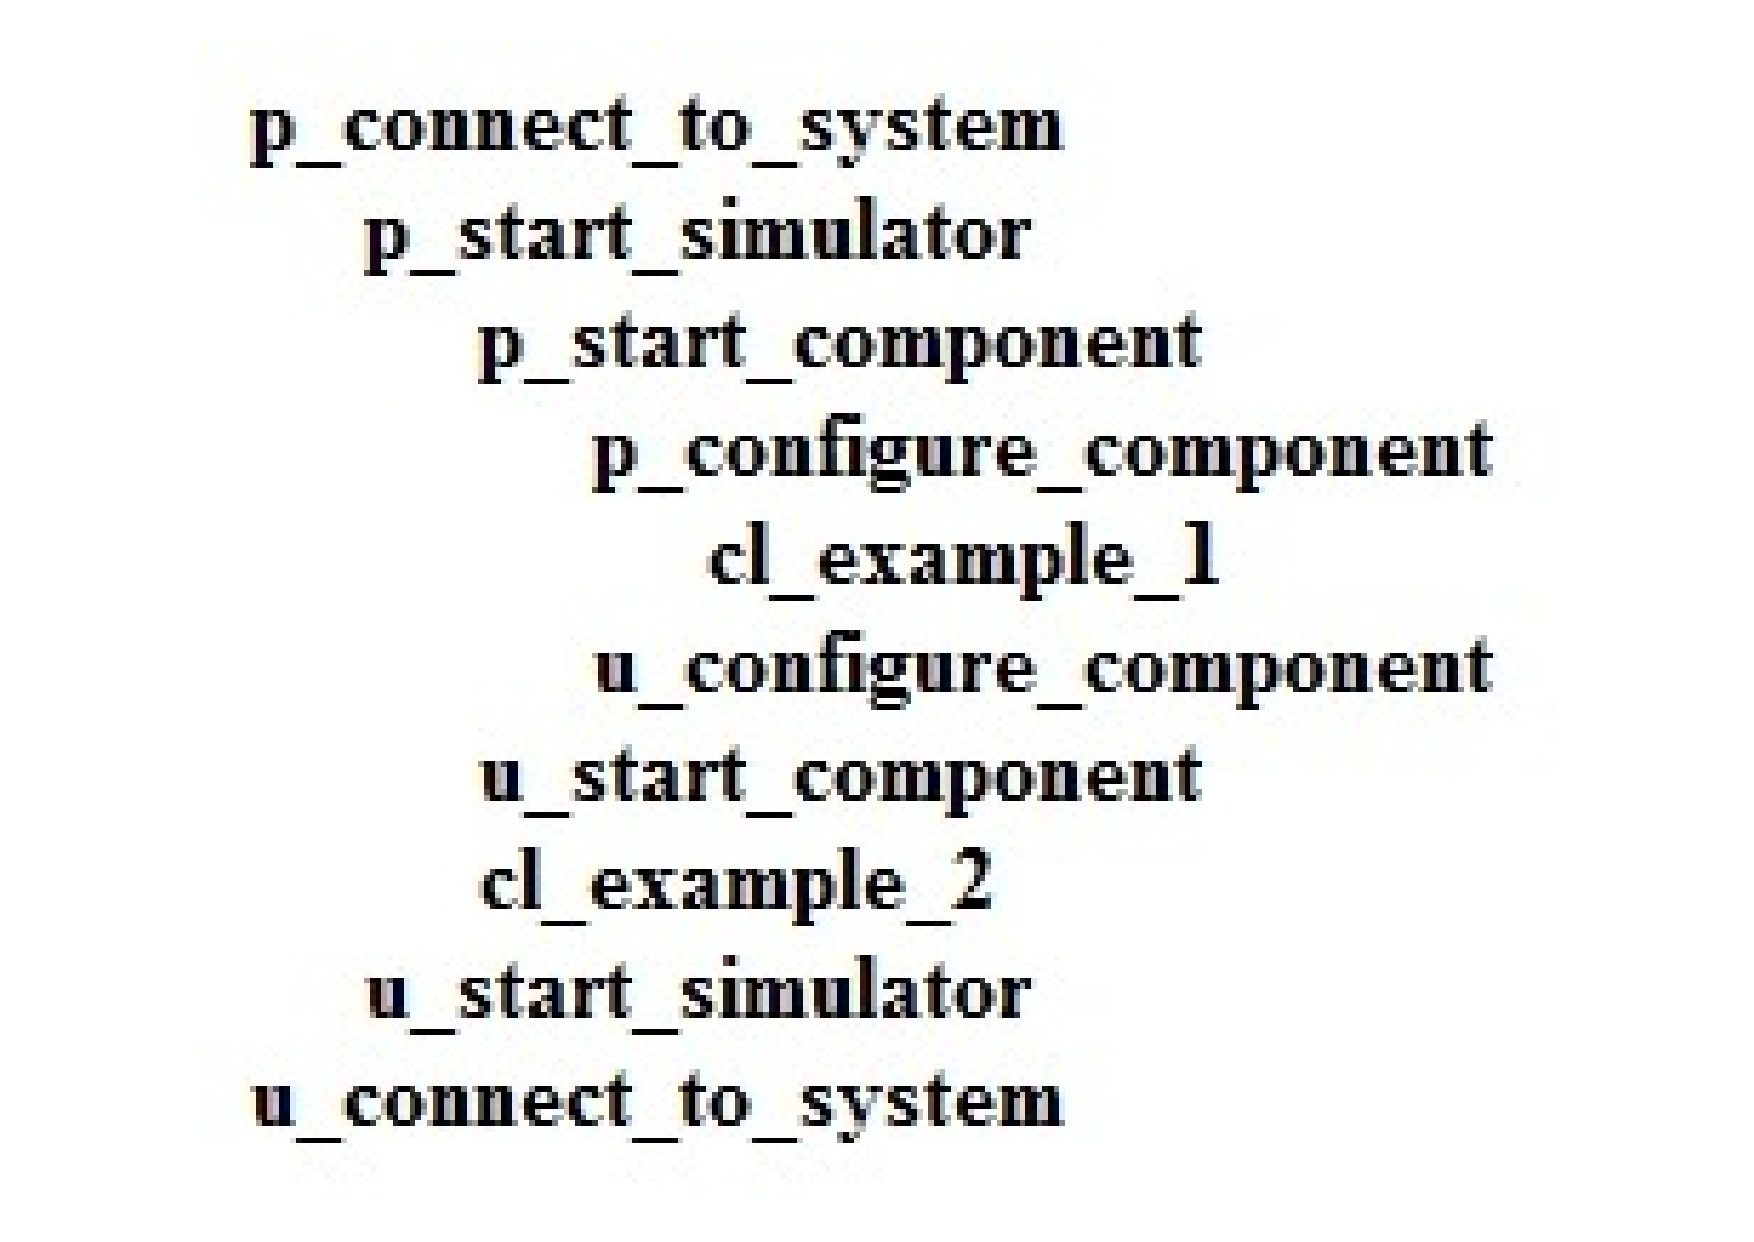
\includegraphics[scale=0.25]{ukazka_planu}
    \caption{Ukážka plánu testov}
    \label{figure:ukazka_planu}
    \end{center}
\end{figure}

Jednotlivé testy sa potom vykonávajú sekvenčne. Výhodou tohoto prístupu je, že v~prípade, že sa zmena konfigurácie nepodarila,
daný cluster môžeme preskočiť, a~tým ušetriť čas na dokončenie testovania. 
Test je úspešný, pokiaľ skončí s~nulovou návratovou hodnotou. V~opačnom prípade je test neúspešný. 
Ďalšou výhodou je znovupoužiteľnosť prerekvizít. 
Jednotlivé prerekvizity totiž môžeme kombinovať a~využiť ich tak pre potreby rôznych typov scenárov pre testy. 

Na obrázku \ref{figure:ukazka_planu} je znázornený príklad dvoch clusterov, pričom každý z~nich vyžaduje iné nastavenie systému. 
Z~obrázku je vidno, že pre potreby clusteru \texttt {cl\_example\_1} je nutné vykonať prerekvizity \texttt{p\_connect\_to\_system}, 
\texttt{p\_start\_component}, \texttt{p\_start\_simulator} a~\texttt{p\_configure\_component},
pričom clusteru \texttt{cl\_example\_2} stačia prerekvizity \texttt{p\_connect\_to\_system} a~\texttt{p\_start\_simulator}.
Nakoľko cluster \texttt{cl\_example\_2} sa spúšťa až za clusterom \texttt{cl\_example\_1}, je nutné vrátiť zmeny systému, ktoré vykonali prerekvizity 
\texttt{p\_start\_component} a~\texttt{p\_configure\_component} pomocou odrekvizít \texttt{u\_start\_component} a~\texttt{u\_configure\_component}.
Jednotlivé prerekvizity na seba môžu, ale nemusia byť závislé, a~preto sa poradie spúšťania prerekvizít môže pre clustre meniť.
Príkladom závislosti môžu byť 2 prerekvizity, kde jedna prerekvizita zapína nejakú súčasť systému s~jeho defaultnými nastaveniami a~druhá prerekvizita 
tieto nastavenia mení. V~druhej prerekvizite môže byť preto nastavené, aby sa spustila, iba ak sa predtým úspešne splnila prerekvizita na zapnutie 
časti systému.
Plánovačka testov sa snaží plánovať jednotlivé clustre za seba tak, aby sa nemuseli nutne vykonať všetky prerekvizity a~odrekvizity pre každý cluster zvlášť.
Znamená to, že ak majú dva clustre podobné prerekvizity, tak sa tieto clustre naplánujú tak, že sa podobné prerekvizity združia a~spúšťajú sa spravidla len raz. 
Táto vlasnosť je znázornená na obrázku \ref{figure:ukazka_zdruzovania}. 
\begin{figure}[h]
    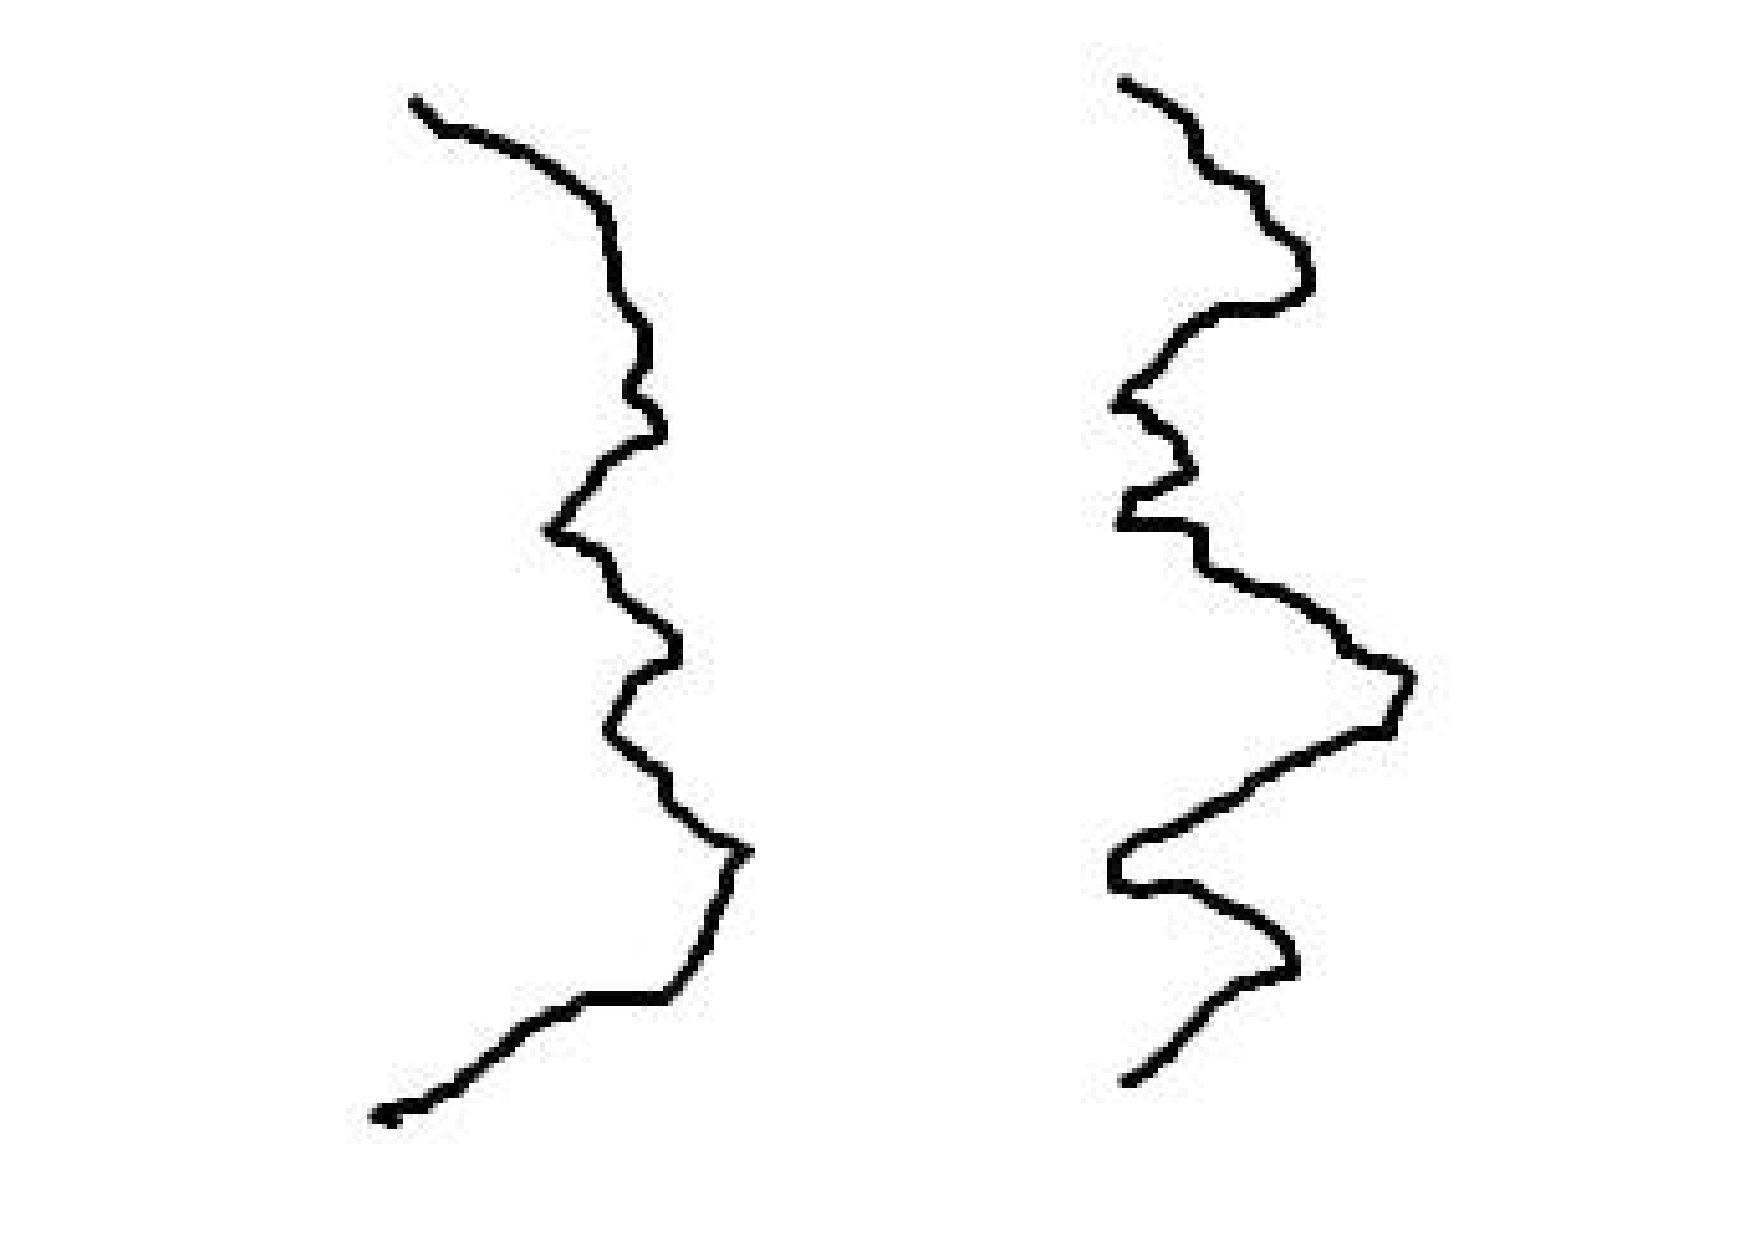
\includegraphics[scale=0.25]{ukazka_zdruzovania}
    \caption{Ukážka vlastnosti združovania testov}
    \label{figure:ukazka_zdruzovania}
\end{figure}

V~regresnej sade sa bežne nachádzajú clustre, ktoré majú rovnakú množinu prerekvizít. Takéto clustre sa radia za seba, aby sa minimalizovalo
spúšťanie prerekvizít a~odrekvizít, ktoré majú ajtak spoločné. Neplatí teda pravidlo, že každý cluster má svoju vlastnú unikátnu prerekvizitu.
Tabuľky \ref{table:tabulka_pomer_mco} a~\ref{table:tabulka_pomer_smsc} zobrazujú prehľad testov v~regresnej sade dvoch najväčších produktoch,
ktoré sa vo firme Acision testujú.

\begin{table}
  \begin{center}
    \begin{tabular}{| l | l | l |}
    \hline
    typ testu & počet testov & priemerný čas vykonávania testu v~sekundách\\ \hline
    cluster & 1000 & 20 \\ \hline
    prerekvizita & 250 & 25 \\ \hline
    odrekvizita & 250 & 13 \\
    \hline
    \end{tabular}
    \label{table:tabulka_pomer_mco}
    \caption{Prehľad jednotlivých testov v~produkte MCO}
  \end{center}
\end{table}

\begin{table}
  \begin{center}
    \begin{tabular}{| l | l | l |}
    \hline
    typ testu & počet testov & priemerný čas vykonávania testu v~sekundách \\ \hline
    cluster & 2000 & 15 \\ \hline
    prerekvizita & 550 & 10 \\ \hline
    odrekvizita & 550 & 12 \\
    \hline
    \end{tabular}
    \label{table:tabulka_pomer_smsc}
    \caption{Prehľad jednotlivých testov v~produkte SMSCv5}
  \end{center}
\end{table}

Medzi ďalšie výhody tohto plánovača testov patrí možnosť špecifikovania pravidiel, s~akými sa budú dané testy spúšťať.
Je napríklad možné nastaviť clusteru zoznam clusterov, takzvaných preoptov, ktoré musia byť úspešne vykonané ešte predtým, ako sa vykoná samotný
cluster. V~prípade, že sa aspoň jeden z~týchto preoptov nevykoná úspešne, cluster sa preskočí.
Výhoda tohto prístupu je v~tom, že ak zo sady testov, ktoré testujú podobnú funkcionalitu, neprejde najzákladnejší test,
môžeme predpokladať, že všetky pokročilejšie testy by neprešli tiež, a~preto ich môžeme preskočiť.

Jednotlivé testy môžeme označovať vhodne zvoleným názvom nejakej funkcionality, pričom môžeme využiť vlastnosť 
plánovača, ktorý nám naplánuje len testy zvolené týmto názvom. Týmto spôsobom môžeme v~regresnej sade vytvárať isté logické celky,
ktoré v~prípade potreby môžeme otestovať samostatne. Pre regresný beh je použitá funkcionalita {\it all}, ktorá združuje 
všetky testy, ktoré nie sú explicitne označené funkcionalitou {\it notall}. 

Za zmienku patrí aj možnosť označiť niektoré testy do kategórie označenej ako {\it known bugs}.
Testy z~tejto kategórie sú v~prípade zlyhania vylúčené zo zoznamu testov, ktoré zlyhali.
Typicky sa takto označujú testy, ktoré úspešne testujú nejakú funkcionalitu, ale vďaka nejakej nesúvisiacej chybe 
dopadajú neúspechom. Takýmto testom je možné explicitne uviesť rozsah verzie softvéru, v~ktorom je tento test chybný.

Každý test má svoj zdrojový kód v~spomínanom jazyku TCL a~svoju vlastnú hlavičku, ktorá obsahuje informácie potrebné pre identifikovanie testu a~jeho úspešné zaradenie do regresnej sady.
Zdrojové kódy testov sú logicky rozdelené a~umiestnené v~súboroch začínajúcich predponou {\it CL-} a~s~príponou {\it .tcl}, napríklad {\it CL-SMPP.tcl} alebo {\it CL-GSM.tcl}.
Hlavičky testov môžu byť taktiež logicky delené na niekoľko celkov a~začínajú predponou {\it TEST.}, napríklad {\it TEST.ALL} alebo {\it TEST.REVIEW\_23}.
Takýmto spôsobom sú napríklad delené testy, ktoré prešli kontrolou a~sú úspešne zaradené do regresnej sady (súbor {\it TEST.ALL}) a~testy, ktoré sú do regresnej sady zaradené, ale
zatiaľ neboli nikým skontrolované (súbor {\it TEST.REVIEW\_23}).

Hlavička každého testu obsahuje nasledovné informácie:
\begin{itemize}
\item \textbf{Name -} názov testu
\item \textbf{Description -} stručný popis, čo daný test vykonáva. 
\item \textbf{odrekvizita -} je test, ktorý vracia zmeny systému spôsobené jej vlastnou prerekvizitou. Každá odrekvizita je pomenovaná
pomocou prefixu {\it u\_}. 
\item \textbf{test -} je cluster, prerekvizita alebo odrekvizita.
\item \textbf{pre -} je množina všetkých prerekvizít, ktoré musia byť splnené, aby sa daný cluster mohol spustiť.
\item \textbf{preopt -} je množina všetkých clusterov, ktoré musia byť úspešne vykonané, aby bolo možné daný cluster vykonať.  
\end{itemize}

Táto sekcia obsahovala zhrnutie toho, akým princípom funguje plánovač testov vytvorený firmou Acision.
Na záver si ešte uvedieme zoznam výhod a~nevýhod použitia tohoto nástroja.

\noindent Výhody:
\begin{itemize}
\item jednoduché zaradenie nového testu do regresnej sady
\item možná znovupoužiteľnosť prerekvizít
\item náväznosť jednotlivých testov
\item 
\item 
\item 
\end{itemize} 

\noindent Nevýhody:
\begin{itemize}
\item 
\item  
\item jednotlivé testy v~prípade chyby systému nemusia úspešne túto chybu obnoviť, a~môžu spustiť lavínu chýb ktoré by inak nenastali 
\item v~prípade, že sa konfiguračné zmeny v~odrekvizitách úspešne neobnovia, dochádzame k~neodpovedajúcim výsledkom z~testovania
\item 
\item 
\end{itemize}

\chapter{Návrh riešenia}
Táto kapitola sa zaoberá základným návrhom
\section{Možnosti rozdeľovania testov}
\section{Komunikácia medzi jednotlivými plánovačmi testov}
\section{Interpretácia výsledkov}
\section{Riešenie nových typov problémov}


\chapter{Implementácia}
V~tejto kapitole sa budeme venovať 
\section{Použité technológie}
\section{Delenie testov na podmnožiny}
\section{Spúšťanie podprocesov a~komunikácia s~nimi}
\section{Sledovanie aktuálneho stavu testovania}
\section{Zbieranie a~vyhodnocovanie výsledkov}
\section{Optimalizácie rozdeľovania testov}


\chapter{Zhodnotenie dosiahnutých výsledkov}
\section{Prínos použitia paralelného plánovača testov}
\section{Porovnanie jednotlivých optimalizácií}


\chapter{Záver}
\section{Zhrnutie}
\section{Možnosti ďalšieho vývoja}

%=========================================================================
